\documentclass{article}

\usepackage{graphicx}
\usepackage{amsmath}

\title{Local recomputation of strongly-connected components}

\begin{document}

\begin{figure}
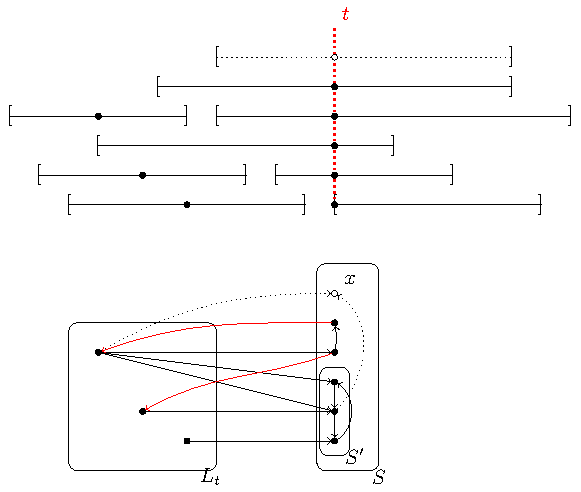
\includegraphics[width=\textwidth]{tikz_figures/sub_instance.pdf}
\caption{Illustration of a situation where an easy SCC-based decision
may be taken regarding the optimal ordering of 
the sub-instance associated to $t$ and $S\setminus\{x\}$. Indeed, in this
sub-instance, because $x$ is not in the instance, $S'$ is a strongly connected
component that can be solved separately and put at the end of an optimal order.
}
\label{illustration_situation}
\end{figure}

We recall that the Kobayashi-Tamaki dynamic programming scheme uses a table
indexed by $(t,S)$, with $t$ a position (see Figure~\ref{illustration_situation})
and $S\subseteq M_t$, with $M_t$ the set of vertices whose intervals intersect
$t$. If $t$ is the opening position of the interval of a vertex (as in Figure~\ref{illustration_situation}), then the entry may be computed with:
$$OPT[t,S] = \min_{x\in S} \left[OPT[t,S\setminus\{x\}]+c(L_t\cup S\setminus\{x\},x)\right]$$

where $L_t$ is the set of vertices whose intervals lay entirely before
$t$. This formula relies on the fact that an optimal order
for the sub-graph induced by $L_t\cup S$ and their neighbors
must end with an element of $S$ (because $t$ is an opening
position for a vertex that must come after $L_t$.

A so-far-undetected optimization is that, in the sub-instance $S\setminus\{x\}$,
because $x$ has been removed, it is possible that a subset $S'\subset S$
has become a separate strongly connected component. If this the case,
and optimal order for $L_t\cup S\setminus \{x\}$ would be:
$$\text{\tt optimal\_order}(L_t\cup S\setminus\{x\} = \text{\tt optimal\_order}(L_t\cup S\setminus\{x\}\setminus S') \cdot \text{\tt optimal\_order}(S')$$
and for the optimal number of crossings: 
$$OPT[L_t\cup S\setminus\{x\}] = OPT[L_t\cup\setminus\{x\}\setminus S']+OPT[S']+\text{\tt crossings}(L_t\cup\setminus\{x\}\setminus S',S')$$

\paragraph{Implementation} Note that we may compute the strongly connected
components on a compacted graph in which $L_t$ has been merged into a single
vertex. Note also that this rule may only be used in a memoization implementation
of the Kobayashi-Tamaki algorithm, which is not the current implementation.

\end{document}
